\providecommand{\main}{..}
\documentclass[\main/main.tex]{subfiles}
\begin{document}
\chapter{Technologies}
\section{Cluster computing}
Modern applications require to deal with immense amount of data as quick as possible. In many of these applications, data is extremely regular, so there is opportunity to exploit parallelism. Examples of possible applications are:
\begin{enumerate}
    \item Web page ranking;
    \item Social networks analysis;
    \item Parallelizable computations.
\end{enumerate}
This parallelization is not achieved using a super computer that can handle the computation, but is achieved using ``computing clusters''. Computing clusters are large collections of commodity hardware, including conventional processors, connected by Ethernet network. The software stack begins with a new form of file system, called a ``distributed file system'', which features much larger units than the disk blocks in a conventional operating system. Distributed file systems also provide replication of data or redundancy to protect against the frequent media failures that occur when data is distributed over thousands of low-cost compute nodes \cite{leskovec_rajaraman_ullman_2020}.

\subsection{Big data}
Big data \cite{Gandomi2015BeyondTH} is high-volume, high-velocity and/or high-variety information assets that demand cost-effective, innovative forms of information processing that enable enhanced insight, decision making, and process automation \cite{bigdatagartner}.
\begin{enumerate}
    \item \textbf{Volume}: the magnitude of data. Big data sizes could be terabytes or even petabytes.
    \item \textbf{Variety}: the structural heterogeneity in a dataset. Data could be structured, semi-structured or unstructured.
    \item \textbf{Velocity}: data generation rate. Data analysis speed is a strongly connected concept: the higher the velocity, the higher the needed analysis speed.
\end{enumerate}
Other mentioned dimensions that are not part of the ``core'' definition:
\begin{enumerate}
    \item \textbf{Veracity}: the unreliability of some data sources. For example, social media sentiments are an uncertain data source, because they imply human judgement.
    \item \textbf{Variability}: the variation in data flow rates. Data could be produced by sources at not constant rates.
    \item \textbf{Complexity}: the heterogeneity of data sources. Being generated through a myriad of sources, big data must be cleaned and connected in order to be used.
    \item \textbf{Value}: the importance of big data. Being characterized by a ``low value density'', a big quantity must be analyzed in order to obtain an high value and be remunerative.
\end{enumerate}
\subsection{Distributed file system}
To exploit cluster computing, data must be organized differently from the conventional file systems of single computers. This new organization is called Distributed file system (DFS) and is used as follows:
\begin{enumerate}
    \item files can be very large, up to terabytes in size;
    \item files are rarely updated. They are read as input for calculation and possibly additional data is appended to files.
\end{enumerate}
Files are divided into chunks. Chunks are replicated on different computer nodes. A collection of several computer nodes connected by the same network switch constitutes a rack. If chunks are replicated on different racks, like in Figure \ref{fig:racks_dfs}, a rack failure won't cause any data loss.
Examples of DFS are:
\begin{enumerate}
    \item Google File System (\emph{GFS}) \cite{GhemawatSanjay2003TheGF}, the first of the class;
    \item Hadoop Distributed File System (\emph{HDFS}) \cite{Shvachko2010TheHD}, an open-source DFS used with Hadoop;
    \item Colossus \cite{10.1145/2491245}, an improved version of GFS.
\end{enumerate}
\subsection{Hadoop}
Hadoop is an open source framework overseen by Apache Software Foundation which is written in Java for storing and processing of huge datasets with the cluster of commodity hardware.
\subsubsection{History}
Hadoop was created by Doug Cutting and Mike Cafarella in 2005. It was originally developed to support distribution for the Nutch search engine project. Apache Nutch project was the process of building a search engine system that can index 1 billion pages. After a lot of research on Nutch, Cutting and Cafarella concluded that such a system will cost around half a million dollars in hardware, and along with a monthly running cost of \$30000 approximately. \\
In 2003 Google solved half of their problem: releasing a paper about GFS \cite{GhemawatSanjay2003TheGF}, supplying a solution for the problem of storing very large files which were being generated because of web crawling and indexing processes. \\
In 2004 Google again released a paper about a distributed computation engine called MapReduce \cite{Dean2004MapReduceSD}, which was the solution of processing those large datasets. Cutting and Cafarella started implementing Google’s techniques (GFS and MapReduce) as open-source in the Apache Nutch project. 
In 2006, while working at Yahoo!, he separated the distributed computing parts from Nutch and formed a new project Hadoop with a large team of engineers working on this project. \\
In 2008, Yahoo! released Hadoop as an open source project to ASF(Apache Software Foundation). And in July of 2008, Apache Software Foundation successfully tested a 4000 node cluster with Hadoop. \\
In 2009, Hadoop was successfully tested to sort a PB (PetaByte) of data in less than 17 hours for handling billions of searches and indexing millions of web pages. \\
In December of 2011, Apache Software Foundation released Apache Hadoop version 1.0. \\
Currently, there is Apache Hadoop version 3.3.x which released in June 2021 \cite{hadoop_history}.
\subsubsection{Architecture} Apache Hadoop is a framework for running applications on large clusters built of commodity hardware. The Hadoop framework transparently provides applications for both reliability and data motion. Hadoop implements a computational paradigm named MapReduce, where the application is divided into many small fragments of work, each of which may be executed or re-executed on any node in the cluster. MapReduce works on YARN (Yet Another Resource Negotiator), which performs 2 operations that are Job scheduling and Resource Management. The Purpose of Job scheduler is to divide a big task into small jobs so that each job can be assigned to various slaves in a Hadoop cluster and Processing can be Maximized. Job Scheduler also keeps track of which job is important, which job has more priority, dependencies between the jobs and all the other information like job timing, \dots And the use of Resource Manager is to manage all the resources that are made available for running a Hadoop cluster.  In addition, it provides a distributed file system (HDFS) that stores data on the compute nodes, providing very high aggregate bandwidth across the cluster. Both MapReduce and the Hadoop Distributed File System are designed so that node failures are automatically handled by the framework \cite{hadoop} \cite{hadoop_arch}.

\subsection{HDFS}
HDFS relies on a \emph{master-slave} architecture composed by a master server, the \emph{NameNode}, and from several slave server, the \emph{DataNodes}, generally one per node in the cluster. The NameNode manages the file system namespace and regulates access to files by clients. Each DataNode manages storage attached to the nodes that they run on. In Figure \ref{fig:hdfs_architecture}, is visible a simple schema of HDFS architecture.
\begin{figure}[H]
    \centering
    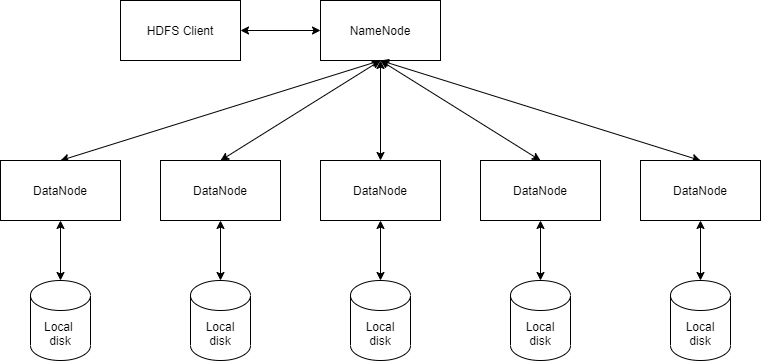
\includegraphics[scale=.5]{images/cluster_computing/hdfs_architecture.png}
    \caption{HDFS  architecture}
    \label{fig:hdfs_architecture}
\end{figure}
\subsubsection{HDFS Blocks} 
HDFS breaks down a file into smaller units. Each of these units is stored on different machines in the cluster. This, however, is transparent to the user working on HDFS. To them, it seems like storing all the data onto a single machine. These smaller units are the blocks in HDFS.
\subsubsection{HDFS NameNode}
NameNode is the master node that runs on a separate node in the cluster.
Manages the filesystem namespace which is the filesystem tree or hierarchy of the files and directories.
Stores information like owners of files, file permissions, \dots for all the files.
It is also aware of the locations of all the blocks of a file and their size.
All this information is maintained persistently over the local disk in the form of two files: Fsimage and Edit Log.
Fsimage stores the information about the files and directories in the filesystem. For files, it stores the replication level, modification and access times, access permissions, blocks the file is made up of, and their sizes. For directories, it stores the modification time and permissions.
Edit log on the other hand keeps track of all the write operations that the client performs. This is regularly updated to the in-memory metadata to serve the read requests.
Whenever a client wants to write information to HDFS or read information from HDFS, it connects with the NameNode. The NameNode returns the location of the blocks to the client and the operation is carried out.
\subsubsection{HDFS DataNode}
DataNode are the worker nodes. They are inexpensive commodity hardware that can be easily added to the cluster. Datanodes are responsible for storing, retrieving, replicating, deletion, \dots of blocks when asked by the NameNode. They periodically send heartbeats to the NameNode so that it is aware of their health. With that, a DataNode also sends a list of blocks that are stored on it so that the NameNode can maintain the mapping of blocks to DataNodes in its memory.

\subsubsection{Rack awareness} HDFS stores replicated datablocks in at least two different racks in order to improve data availability, reliability and network bandwidth utilization. If the so called replication factor is three, a block is replicated on the local rack and two more replicas are placed in a same remote rack. This allows data recovery in case of connection loss among nodes. The inability to reach a rack (e.g. network problems) doesn't cause a big data loss because data are replicated over different racks, so lost blocks are read from the remaining rack and replicated again in order to guarantee availability, reliability and network bandwidth utilization. In Figure \ref{fig:racks_dfs} is visible the rack organization of a DFS.
\begin{figure}[H]
    \centering
    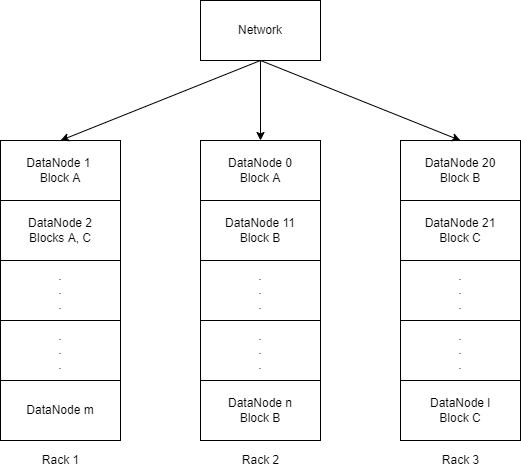
\includegraphics[scale=.6]{images/cluster_computing/racks_dfs.png}
    \caption{HDFS rack architecture}
    \label{fig:racks_dfs}
\end{figure}

\subsection{MapReduce}
MapReduce \cite{Dean2004MapReduceSD} is a distributed computing framework that is used to manage many large-scale, parallel computations in a way that is tolerant of hardware faults. Typically the compute nodes and the storage nodes are the same, that is, the MapReduce framework and the HDFS are running on the same set of nodes. This configuration allows the framework to effectively schedule tasks on the nodes where data is already present, resulting in very high aggregate bandwidth across the cluster, increased computational performances and efficiency. A MapReduce computation consists of:
\begin{enumerate}
    \item Map task: takes in input one or more data blocks and returns a sequence of \emph{key-value} pairs;
    \item Reduce task: combines all the values associated with a key, one key at a time.
\end{enumerate}
The execution overview is visible in Figure \ref{fig:map_reduce}
\begin{figure}[H]
    \centering
    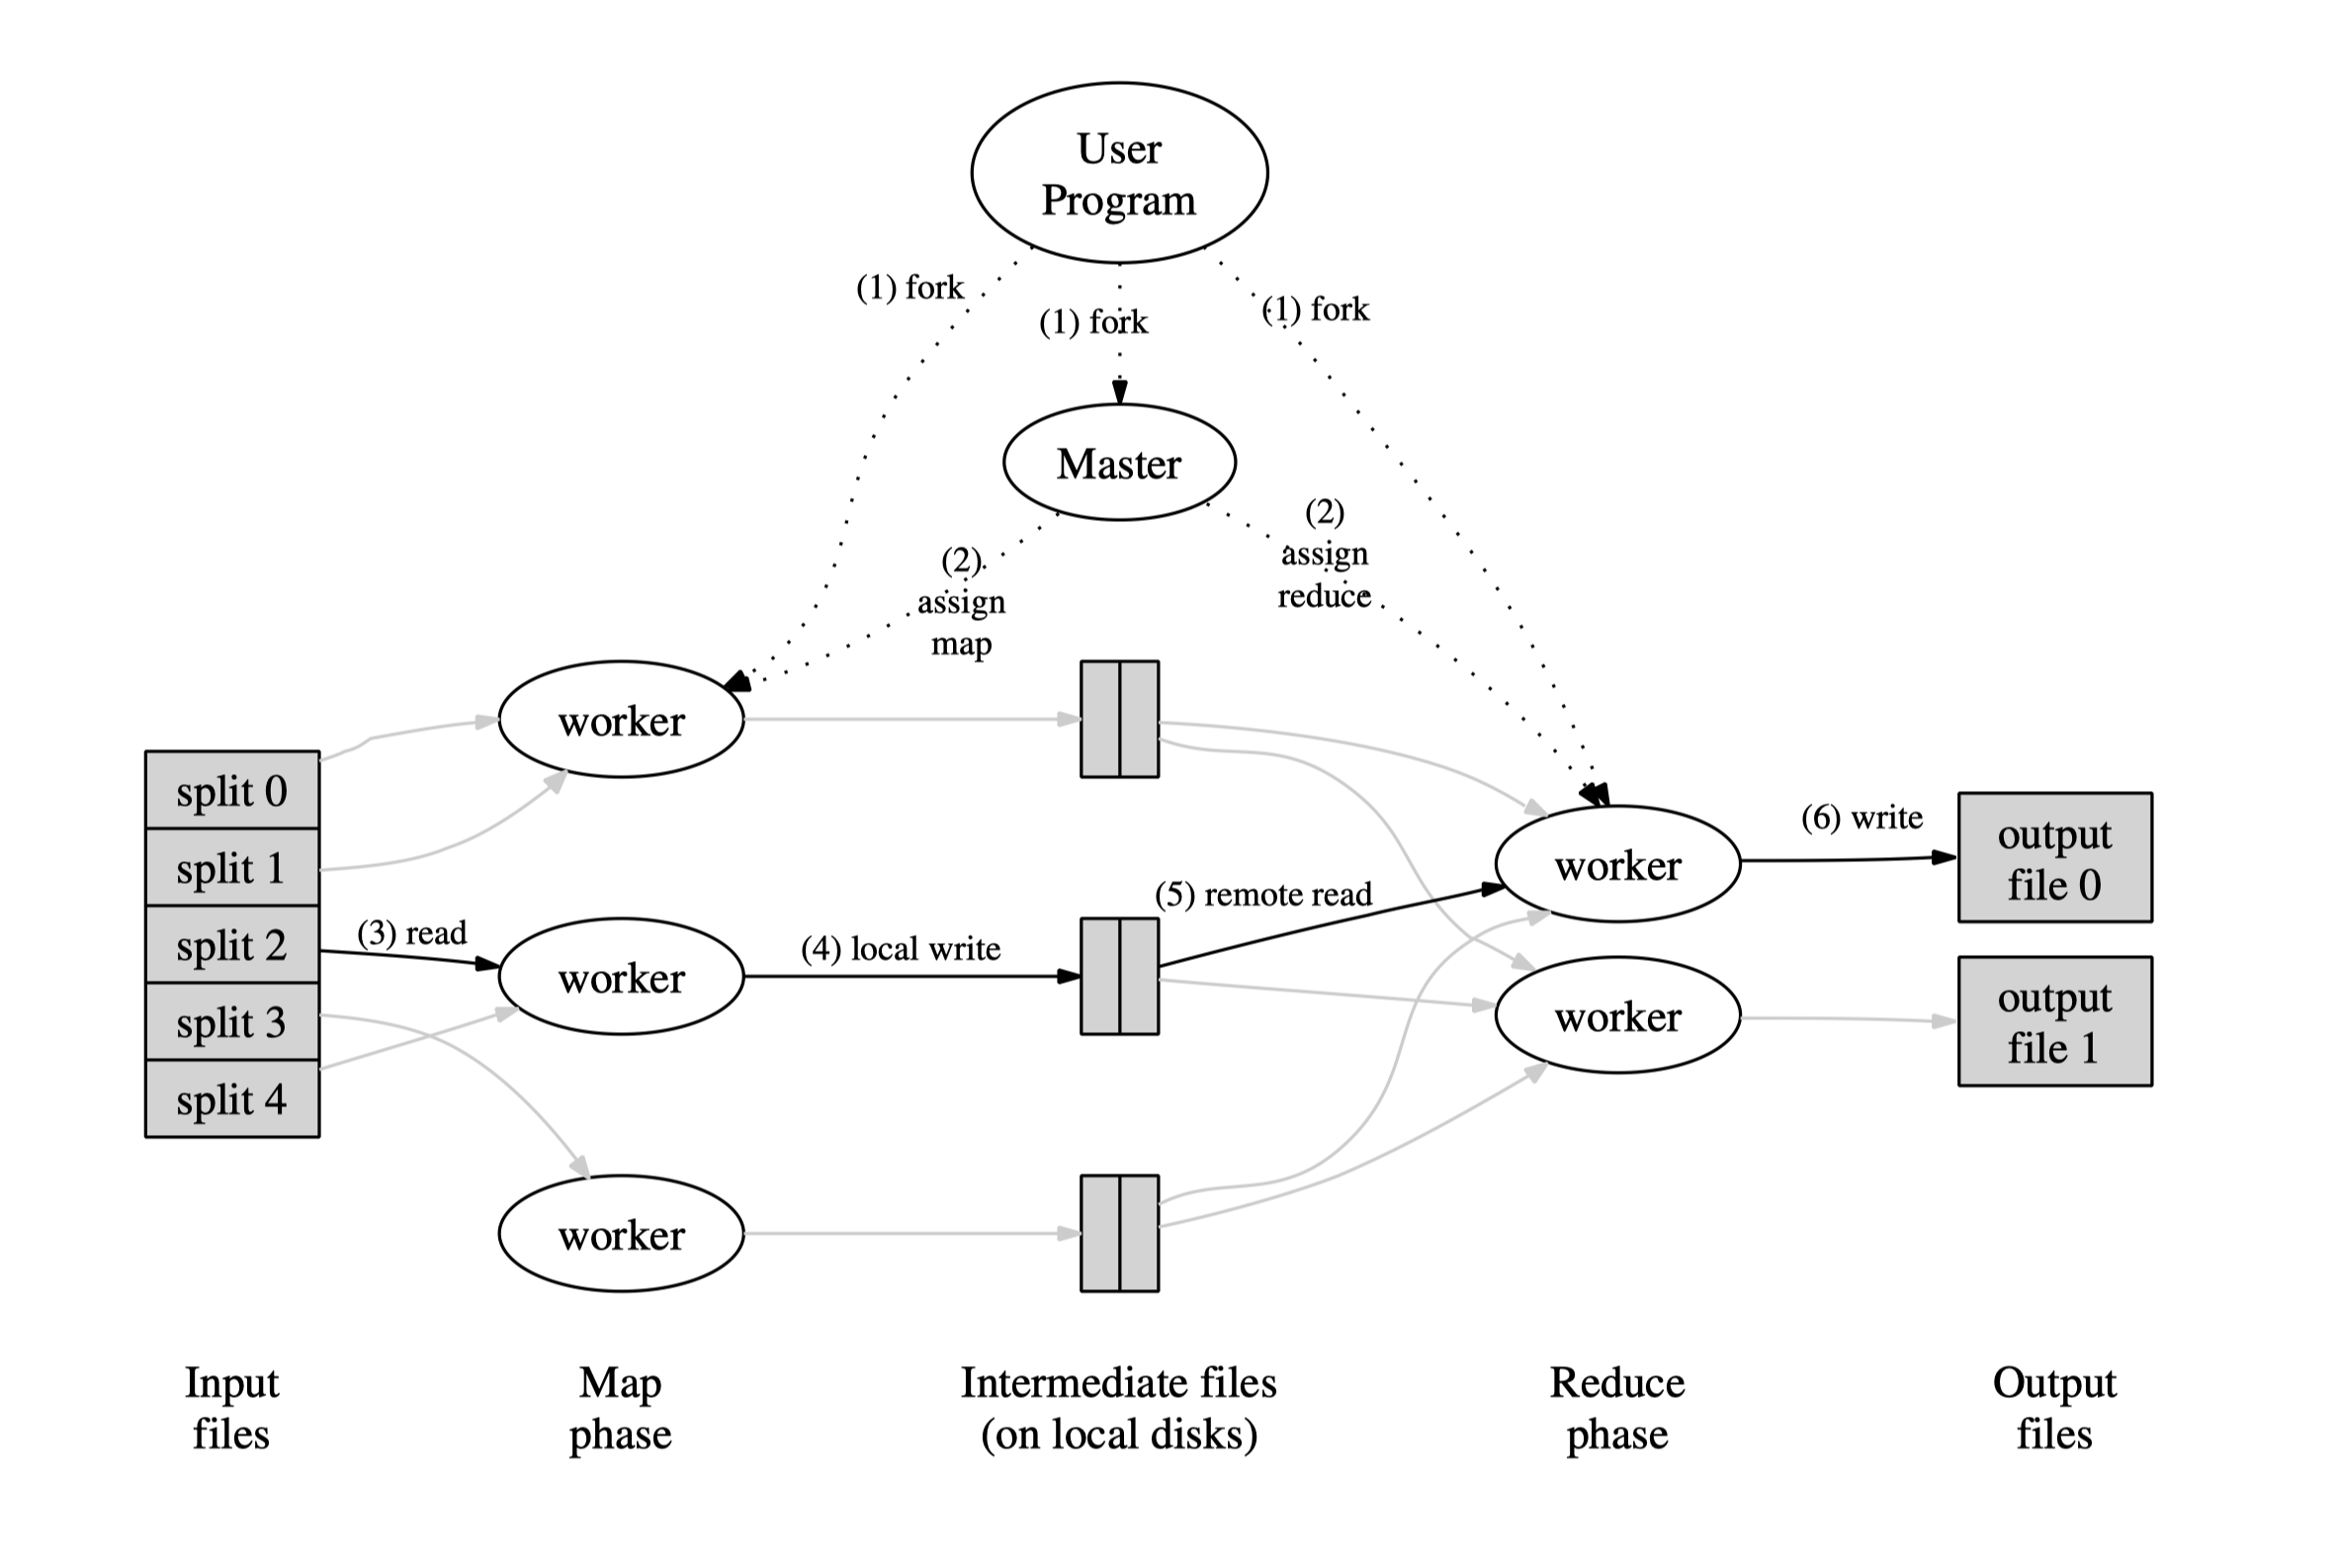
\includegraphics[scale=.35]{images/cluster_computing/map_reduce_schema.png}
    \caption{MapReduce execution overview}
    \label{fig:map_reduce}
\end{figure}
\subsubsection{Map task}
The input files for a Map task are elements of any type: tuple, document, \dots, organized in key-value pair (\emph{k, v})
A block is a collection of elements, and no element is stored across two chunks. 
A Map task produces zero or more key-value pairs, with keys not necessarily uniques.
\subsubsection{Grouping by key}
Once the Map task is over, all key-value pairs are grouped by key, with a single list of values associated to that key.
\subsubsection{Reduce task}
A Reduce task takes as input a pair of key, list of values associated to that key. The task produces a sequence of zero or more key-value pairs as output. The function that is applied on the list of values for a given key is called \emph{reducer}. For each Reduce task, there could be more reducers.
\subsubsection{MapReduce execution}
\begin{enumerate}
    \item The user program forks a Master controller process and some Worker processes at different compute nodes. A Worker handles Map tasks or Reduce tasks, but not both.
    \item According to the user program, the Master creates a given number of Map and Reduce tasks and assigns them to the Workers.
    \item The Master keeps track of the status of each Map and Reduce task (idle, executing, completed) and when a Worker finishes a task, the Master schedules a new task for that Worker.
\end{enumerate}
\subsubsection{Node failure}
\begin{enumerate}
    \item If the Master fails, the entire MapReduce job must be restarted;
    \item If a Map worker fails, all its tasks (even completed), are rescheduled to other workers to complete them eventually;
    \item If a Reduce worker fails, its Reduce tasks will be put to idle status and rescheduled on another Reduce worker.
\end{enumerate}
\subsubsection{Execution management}
The MapReduce framework consists of a single master JobTracker and one slave TaskTracker per cluster-node. The work of JobTracker is to manage all the resources and all the jobs across the cluster and also to schedule each map on the TaskTracker running on the same DataNode since there can be hundreds of DataNodes available in the cluster. The TaskTracker can be considered as the actual slaves that are working on the instruction given by the JobTracker. This TaskTracker is deployed on each of the nodes available in the cluster that executes the Map and Reduce task as instructed by JobTracker.
\subsection{Spark}
Apache Spark is a unified analytics engine for large-scale data processing. It provides high-level APIs in Java, Scala, Python and R, and an optimized engine that supports general execution graphs. It also supports a rich set of higher-level tools including Spark SQL for SQL and structured data processing, MLlib for machine learning, GraphX for graph processing, and Structured Streaming for incremental computation and stream processing \cite{spark}.
\paragraph{Workflow systems} Workflow systems extend MapReduce from the simple two-step workflow (the Map function feeds the Reduce function) to any collection of functions, with an acyclic graph representing workflow among the functions. That is, there is an acyclic flow graph whose arcs $a$ → $b$ represent the fact that function $a$’s output is an input to function $b$ \cite{leskovec_rajaraman_ullman_2020}.
\subsubsection{Data structures}
\paragraph{RDD} Spark is based on Resilient Distributed Datasets (RDD), which is a collection of elements partitioned across the nodes of the cluster that can be operated on in parallel. An RDD is distributed because it can be split into chunks and held at different compute nodes. They're resilient because it's expected that they can be recovered in case of partial or total loss. An RDD can contain elements of any kind, without restrictions \cite{rdd}.
\paragraph{Dataset} A combination of DataFrame and RDD. It provides the typed interface that is available in RDDs while providing the convenience of the DataFrame. The Dataset API is available in the Java and Scala languages \cite{dataset}.
\paragraph{Dataframe} A DataFrame is a Dataset organized into named columns. It is conceptually equivalent to a table in a relational database or a data frame in R/Python, but with richer optimizations under the hood \cite{dataframe}.
\subsubsection{Operations}
Operations in Spark are:
\begin{enumerate}
    \item Transformations: operations applied to an RDD that produce another RDD;
    \item Actions: perform operations on an RDD and pass back the result to the application that called the Spark program.
\end{enumerate}
Spark is and advanced workflow system, because of:
\begin{enumerate}
    \item a more efficient failure handling;
    \item a more efficient way of grouping tasks among compute nodes and scheduling execution of functions;
    \item integration of programming languages features and function libraries;
    \item RDD caching: caching RDDs allows to reuse them in order to reduce computation avoiding recalculating already cached operations, improving performances. 
\end{enumerate}
\subsubsection{Map, FlatMap and Filter}
Differently from MapReduce approach, in Spark Map functions can be applied not only on key-value pairs, but can be applied to any kind of object, producing one object as result. 
FlatMap is the same operation of Map in MapReduce, but without the requirement that all types be key-value pairs. Filter is a transformation that produces an RDD with only the objects that return true to a given predicate.
\subsubsection{Reduce}
Reduce operation is an action. Because of this, it returns a set of values --- possibly smaller then the set taken in input --- and not another RDD. On an RDD, Reduce is applied on every pair of consecutive elements until only one lement remains, that becomes the result of the Reduce operation.
\subsubsection{Spark implementation}
Like Hadoop or other MapReduce implementations, Spark manages large RDDs in the same way: it divides it in splits (MapReduces's chunks) and spreads them to different compute nodes in order to allow parallel computation.
\paragraph{Lazy evaluation}
The first difference from other MapReduce implementations, is that Spark is lazy evaluated: transformations are not applied on an RDD until it is required to do so, typically in correspondence of an action.
\paragraph{Resilience of RDDs}
Performing operations on RDDs creates a \emph{lineage} of those RDDs, so that in case of failure Spark is able to recreate the RDD (or just a split) looking at its lineage.
\newpage
\subsubsection{Other Spark components}
Apart from Spark \emph{core} components, the engine has several other parts important depending on the application scope.
\paragraph{Spark SQL} Spark SQL lets you query structured data inside Spark programs, using SQL. SQL provide a common way to access a variety of data sources, including Hive, Parquet, JSON, \dots.
\paragraph{MLlib} Apache Spark provides a general machine learning library — MLlib — that is designed for simplicity, scalability, and easy integration with other tools. The key benefit of MLlib is that it allows data scientists to focus on their data problems and models instead of solving the complexities surrounding distributed data (such as infrastructure, configurations, and so on). The data engineers can focus on distributed systems engineering using Spark’s easy-to-use APIs, while the data scientists can leverage the scale and speed of Spark core. Spark MLlib is a general-purpose library, providing algorithms for most use cases.
\paragraph{ML Pipelines} When running machine learning algorithms, it involves a sequence of tasks including pre-processing, feature extraction, model fitting, and validation stages. The ML Pipelines is a High-Level API for MLlib that allow the user to execute a sequence of operations, like the ones named before, as a stage of a sequence. This sequence is called \emph{pipeline} and is executed as a whole.
\paragraph{GraphX} GraphX is a component in Spark for graphs and graph-parallel computation. It extends RDDs and exposes a set of operators on graphs (aggregations, joins, structural, property, \dots).
\paragraph{Spark Streaming} Spark Streaming is an extension of the core Spark API that allows data engineers and data scientists to process real-time data from various sources including Kafka, Flume, \dots. This processed data can be pushed out to filesystems, databases, and live dashboards. Extending RDDs, Spark Streaming can be used with any other Spark components like MLlib, Spark SQL, \dots
\subsubsection{Spark on Hadoop}


\section{Transformers}
Until massive adoption of transformer technology, the dominant sequence transduction models were based on complex recurrent or convolutional neural networks that include an encoder and a decoder.
Transformers are a network architecture based only on a attention mechanism, which can be described as mapping a query and a set of key-value pairs to an output (query, keys, values and output are all vectors) \cite{vaswani2017attention}, not explicitly exploiting recurrence and convolution, differently from previously adopted system like recurrent neural networks, long short-term memory and gated recurrent neural networks. Transformers are used to draw global dependencies between input and output. They are used to better handle long-range dependencies within a text. These technologies allow to represent texts in a more semantical way, better capturing context and relations among different parts of the text \cite{vaswani2017attention}. Transformers are the true state of the art in NLP field, since 2018 (year of BERT \cite{devlin2018bert}\cite{bert_blog_post} release) transformers are used in different fields that require a semantic representation of texts. Some examples of Transformer implementations are shortly described here below.
\begin{enumerate}
    \item \textbf{An Image is Worth 16x16 Words: Transformers for Image Recognition at Scale}: in \cite{Dosovitskiy2021AnII}, researchers have applied Transformers directly on sub-portions of an image in order to obtain a representation that can be further used for image classification tasks. Good results are shown when training happens on small datasets.
    \item \textbf{Speech-Transformer: A No-Recurrence Sequence-to-Sequence \\Model for Speech Recognition}: in \cite{Dong2018SpeechTransformerAN}, researchers have presented the Speech-Transformer, a no-recurrence sequence-to-sequence model entirely rely on attention mechanisms to learn the positional dependencies, which can be trained faster and with more efficiency. Results based on the Wall Street Journal speech recognition dataset show that the proposed technology achieves an error rate of 10.9\%, while the whole training process only takes 1.2 days on 1 GPU, significantly faster than the published results of recurrent sequence-to-sequence models. 
\end{enumerate}

\newpage
\subsection{Architecture}
Transformers, like most competitive neural sequence transduction, have an encoder-decoder structure with the encoder mapping an input sequence of symbols $(x_1, \dots, x_n)$ to a continuous representation $z = (z_1, \dots, z_n)$. Given $z$, the decoder generates an output sequence $(y_1, \dots, y_m)$ of symbols one element at a time. In the left and right halves of Figure \ref{fig:transformer_architecture} is shown the fully-connected layers of both encoders and decoders.
\begin{figure}[H]
    \centering
    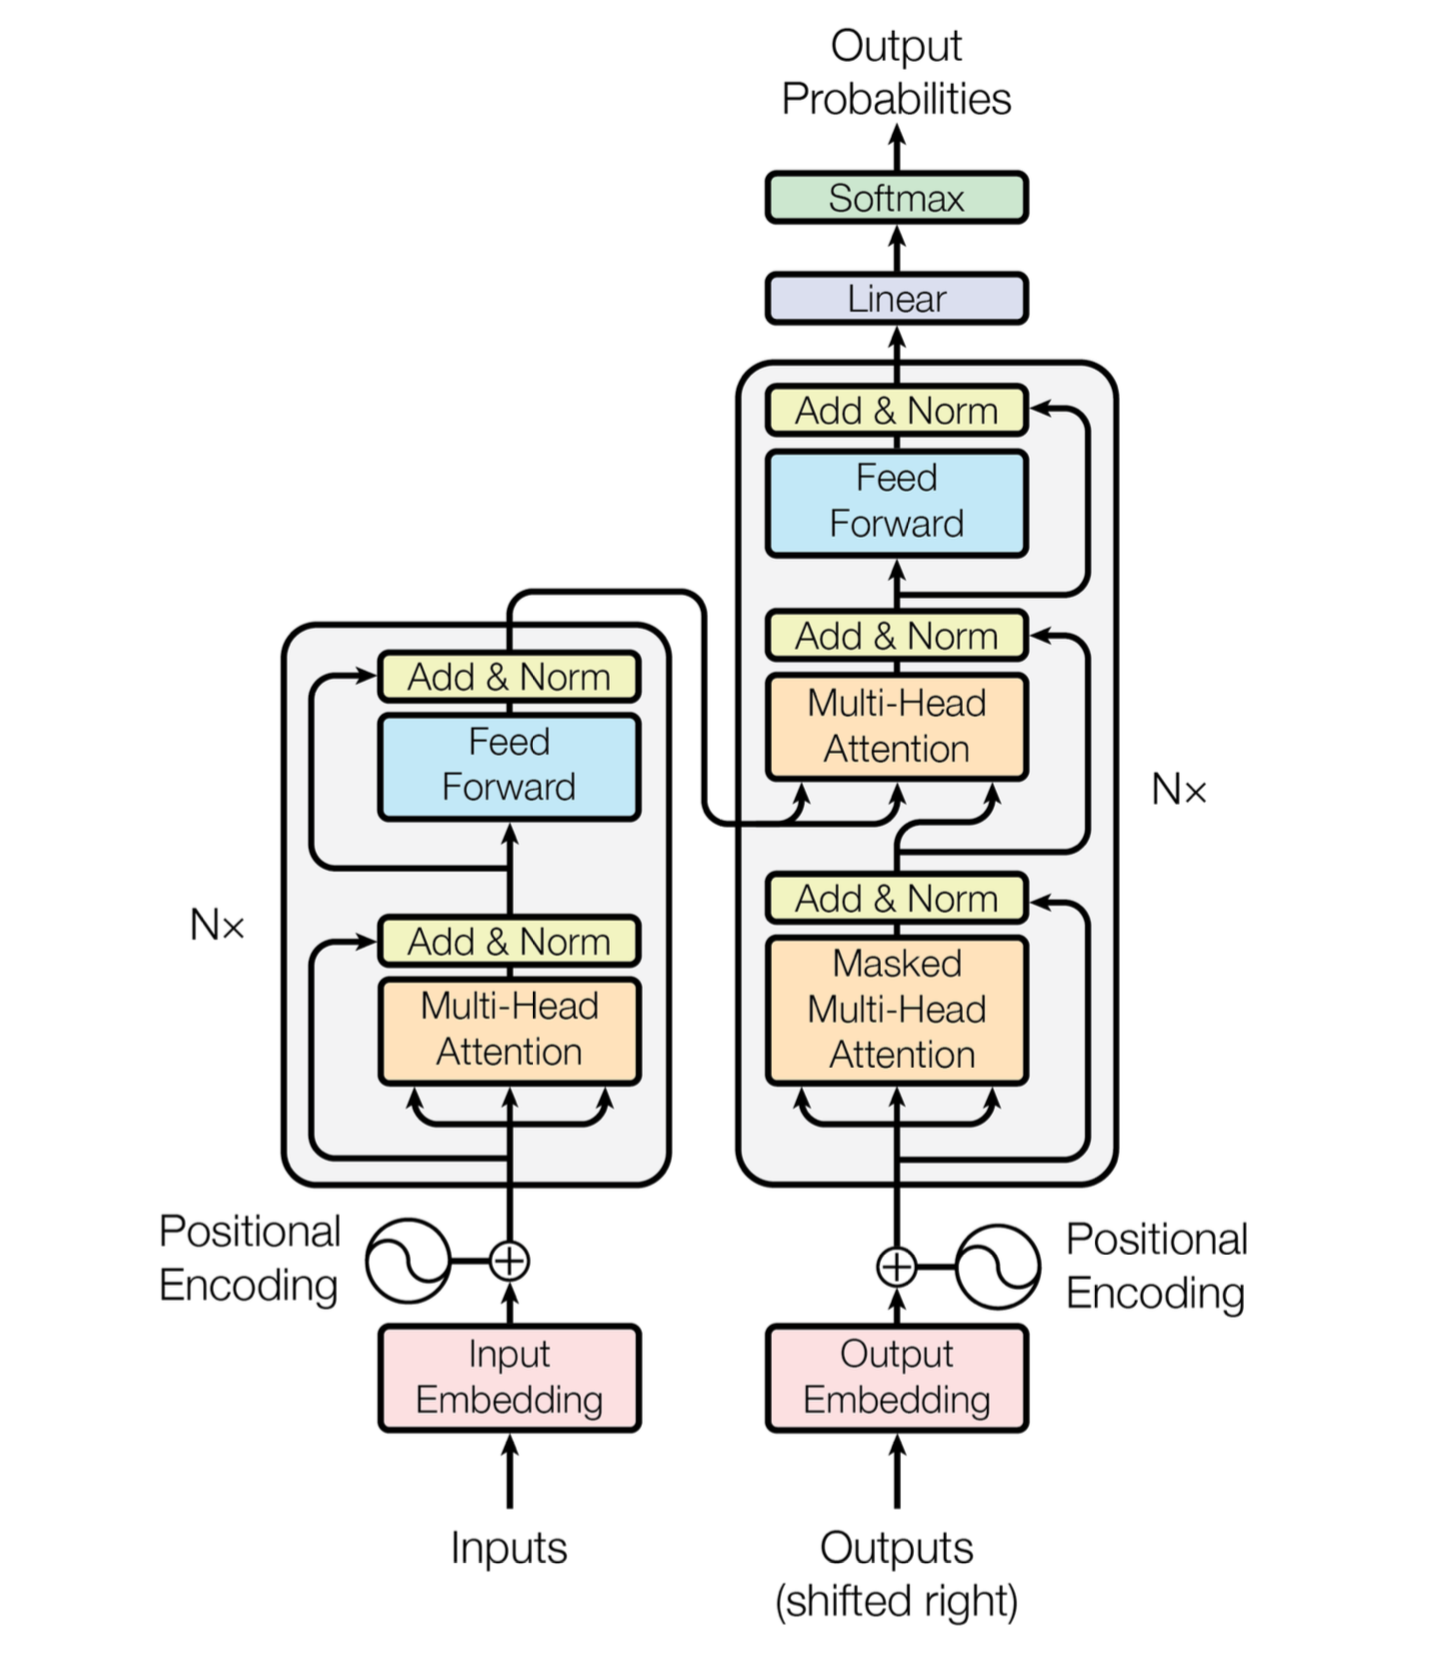
\includegraphics[scale=0.4]{images/transformer/transformer_model_architecture.png}
    \caption{Transformer architecture}
    \label{fig:transformer_architecture}
\end{figure}

\subsection{Encoder}
The encoder from Vaswani's research \cite{vaswani2017attention} is composed of a stack of $N=6$ identical layers, each one has two sub-layers:
\begin{enumerate}
    \item a multi-head self-attention mechanism;
    \item a position-wise fully connected feed-forward network.
\end{enumerate}
A residual connection followed by layer normalization is employed around each sub-layer. All sub-layers in the model produce an output of dimension $d_{model} = 512$.

\subsection{Decoder}
The decoder from Vaswani's research \cite{vaswani2017attention} is composed of a stack of $N=6$ identical layers. The decoder inserts a third sub-layer to the two encoder sub-layer. This sub-layer performs multi-head attention over the output of the encoder stack. The idea behind multi-head attention is to allow the attention function to extract information from different representation subspaces, which would, otherwise, not be possible with a single attention head. Similarly to the encoder, around each of the sub-layers are employed residual connections followed by layer normalization. This kind of masking combined the output embeddings, that are offset by one position, ensures that the predictions for position $i$ can depend only on the known outputs at positions less than $i$. All sub-layers in the model produce an output of dimension $d_{model} = 512$.

\subsection{Attention}
An attention function consists in mapping a query and a set of key-value pairs to an output, where the query, keys, values and output are all term vectors. The main purpose of attention is to estimate the relative importance of the keys term compared to the query term related to the same person or concept. To that end, the attention mechanism takes query $Q$ that represents a vector word, the keys $K$ which are all other words in the sentence, and value $V$ represents the vector of the word. The output is computed as a weighted sum of the values, with weights computed by a compatibility function of the query with the corresponding key.
\subsubsection{Scaled dot-product attention} 
The input consists of queries and keys of dimension $d_k$, and values of dimension $d_v$.
To obtain the weights on the values, the dot product of the query with all keys is performed, dividing each by $\sqrt{d_k}$ and applying a softmax function. The queries, values and keys sets are packed together into $Q$ (queries), $K$ (keys) and $V$ (values) matrices. 
The attention function is computed using $Q$, $K^T$ ($K$ transposed) and $V$ matrices, producing an output matrix in this way:
\begin{center}
    $Attention(Q, K, V) = softmax(\frac{QK^T}{\sqrt{d_k}})V$
\end{center}
Scaled dot-product attention is both faster and more space efficient of two commonly used attention functions: additive attention and dot-product (multiplicative) attention. These performances reachable because of the highly optimized implementation of matrix multiplication code.
\begin{figure}[h!]
    \centering
    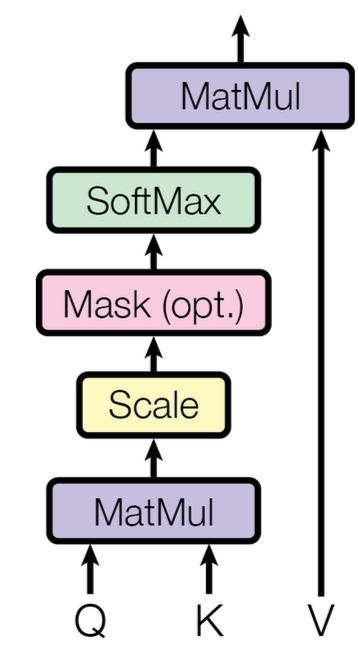
\includegraphics[scale=0.35]{images/transformer/scaled_dot_product_attention.png}
    \caption{Scaled dot-product attention}
    \label{fig:scaled_dot-product_attention}
\end{figure}
\subsubsection{Multi-head attention}
As visible in Figure \ref{fig:multi-head_attention}, queries, values and keys are linearly projected $h$ times, with different learned linear projections to $d_k$, $d_q$ and $d_v$ dimensions respectively. The attention function is performed in parallel on each projection, yielding \mbox{$d_v$-dimensional} output values. These are concatenated and once again projected, resulting in the final values. \\
Multi-head attention allows the model to jointly participate to information from different representation subspaces at different positions. 
\begin{center}
    $\mathrm{MultiHead}(Q, V, K) =\mathrm{Concat}(head_1, \dots, head_h)W^O$\\
    where $head_i = Attention(QW^Q_i, KW^K_i, VW^V_i)$
\end{center}
Where the projections are parameter matrices 
\begin{center}
    $W^Q_i\in\R^{d_{model \times d_k}}, W^K_i\in\R^{d_{model \times d_k}}, W^V_i\in\R^{d_{model \times d_k}}$ and $ W^O_i\in\R^{d_{model \times d_k}}$
\end{center}

\begin{figure}[H]
    \centering
    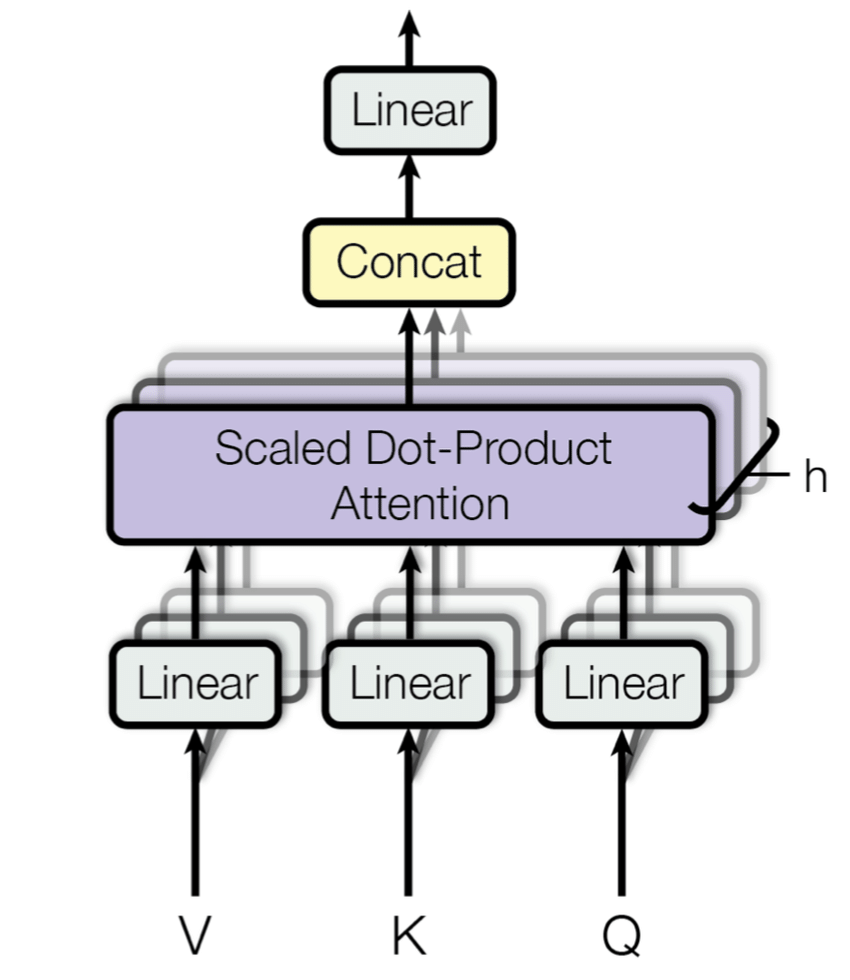
\includegraphics[scale=0.25]{images/transformer/multi-headed_attention.jpeg}
    \caption{Multi-head attention}
    \label{fig:multi-head_attention}
\end{figure}

\subsection{Position-wise Feed-Forward Networks}
Every layer in both encoders and decoders contain a fully connected feed-forward neural network, which is applied to each position separately and identically.
It consists of two linear transformations with a ReLU activation in between.
\begin{center}
    $FFN(x) = \max(0, xW_1 + b_1)W_2 + b_2$
\end{center}
The linear transformations remain the same across different positions, using different parameters on each layer. The dimensionality of input and output is $d_\mathrm{model} = 512$, and the inner-layer has dimensionality $d_\mathrm{ff} = 2048$.

\subsection{Embeddings and softmax}
Learned embeddings are used to convert the input and output tokens to vectors of dimension $d_\mathrm{model}$. The learned linear transformation and softmax function are used to convert the decoder output to predicted next-token probabilities.

\subsection{Positional encodings}
Since the model contains neither recurrence nor convolution, relative or absolute tokens positional encodings are injected in order to make use of the order of the sequence. Positional encodings are added to the input embeddings of the encoder and decoder stacks. They have the same dimension $d_\mathrm{model}$ as the embeddings, so the two can be summed.

\subsection{Self-attention motivations}
In order to understand why self-attention layers are used, it's necessary to compare them with recurrent and convolutional layers. There are three aspects that are important to consider: the total computation complexity per layer, the amount of computation that can be parallelized (intended as the minimum number of sequential operations required) and the path length between long-range dependencies in the network. \\
In terms of computation that can be parallelized, a self-attention layer connects all positions with a constant number of sequentially executed operations, whereas a recurrent layer requires $O(n)$ sequential operations. In terms of computational complexity, self-attention layers are faster than recurrent layers when the sequence length $n$ is smaller than the representation dimensionality $d$, which is most often the case with sentence representations used by state-of-the-art models in machine translations, such as word-piece and byte-pair representations. Table \ref{table:complexity_self_attention} shows the complexity comparison between self attention, recurrence and convolutions from the point of view of maximum path lengths, per-layer complexity and minimum number of sequential operations for different layer types. 

\begin{table}[H]
\centering
\begin{tabular}{||c c c c||} 
 \hline
 Layer type & Comp. per layer & Seq. ops & Max path length \\ [0.5ex] 
 \hline\hline
 Self attention & $O(n^2 \cdot d)$ & $O(1)$ & $O(1)$ \\ 
 \hline
 Recurrent & $O(n \cdot d^2)$ & $O(n)$ & $O(n)$ \\
 \hline
 Convolutional & $O(k \cdot n \cdot d^2)$ & $O(1)$ & $O(log_k(n))$ \\
 \hline
 
\end{tabular}
\caption{Self attention complexity}
 \label{table:complexity_self_attention}
\end{table}


\end{document}